%%%%%%%%%%%%%%%%%%%%%%%%%%%%%%%%%%%%%%%%%%%%%%%%%%%%%%%%%%%%%%%%%
% \documentclass[hyperref={pdfpagelabels=false},compress,table]{beamer} % 在Mac下无法编译
\documentclass[compress,table]{beamer} % 在Mac下使用
% package for font
\usepackage{fontspec}
\defaultfontfeatures{Mapping=tex-text}  %%如果没有它,会有一些 tex 特殊字符无法正常使用,比如连字符。
\usepackage{xunicode,xltxtra}
\usepackage[BoldFont,SlantFont,CJKnumber,CJKchecksingle]{xeCJK}  % \CJKnumber{12345}: 一万二千三百四十五
\usepackage{CJKfntef}  %%实现对汉字加点、下划线等。
\usepackage{pifont}  % \ding{}
% package for math
\usepackage{amsfonts}

% package for graphics
\usepackage[americaninductors,europeanresistors]{circuitikz}
\usepackage{tikz}
\usetikzlibrary{plotmarks}  % placements=positioning
\usepackage{graphicx}  % \includegraphics[]{}
\usepackage{subfigure}  %%图形或表格并排排列
% package for table
\usepackage{colortbl,dcolumn}  %% 彩色表格
\usepackage{multirow}
\usepackage{multicol}
\usepackage{booktabs}
% package for code
\usepackage{fancyvrb}
\usepackage{listings}

% \usepackage{animate}
% \usepackage{movie15}

%%%%%
% setting for beamer
\usetheme{default} % Madrid(常用), Copenhagen, AnnArbor, boxes(白色), Frankfurt,Berkeley
\useoutertheme[subsection=true]{miniframes} % 使用Berkeley时注释本行
\usecolortheme{sidebartab}
\usefonttheme{serif}  %%英文使用衬线字体
% \setbeamertemplate{background canvas}[vertical
% shading][bottom=white,top=structure.fg!7] %%背景色,上25%的蓝,过渡到下白。
\setbeamertemplate{theorems}[numbered]
\setbeamertemplate{navigation symbols}{}  %% 去掉页面下方默认的导航条
\setbeamercovered{transparent}  %设置 beamer 覆盖效果

% 设置标题title背景色
% \setbeamercolor{title}{fg=black, bg=lightgray!60!white}
\setbeamercolor{title}{fg=white, bg=black!70!white}

% 设置每页小LOGO
\pgfdeclareimage[width=1cm]{ouc}{figures/static/ouc.pdf}
\logo{\pgfuseimage{ouc}{\vspace{-20pt}}}

% setting for font
%%\setCJKmainfont{Adobe Kaiti Std}
\setCJKmainfont{SimSun} 
%% \setCJKmainfont{FangSong_GB2312} 
%% \setmainfont{Apple Garamond}  %%苹果字体没有SmallCaps
\setCJKmainfont{SimSun} 
%FUNNY%\setCJKmainfont{DFPShaoNvW5-GB}  %%华康少女文字W5(P)
%FUNNY%\setCJKmainfont{FZJingLeiS-R-GB}  %%方正静蕾体
%FUNNY%\setmainfont{Purisa}
%\setsansfont[Mapping=tex-text]{Adobe Song Std}
     %如果装了Adobe Acrobat,可在font.conf中配置Adobe字体的路径以使用其中文字体。
     %也可直接使用系统中的中文字体如SimSun、SimHei、微软雅黑等。
     %原来beamer用的字体是sans family;注意Mapping的大小写,不能写错。
     %设置字体时也可以直接用字体名,以下三种方式等同:
     %\setromanfont[BoldFont={黑体}]{宋体}
     %\setromanfont[BoldFont={SimHei}]{SimSun}
     %\setromanfont[BoldFont={"[simhei.ttf]"}]{"[simsun.ttc]"}
% setting for graphics
\graphicspath{{figures/}}  %%图片路径
\renewcommand\figurename{图}

% setting for pdf
\hypersetup{% pdfpagemode=FullScreen,%
            pdfauthor={Xiaodong Wang},%
            pdftitle={Title},%
            CJKbookmarks=true,%
            bookmarksnumbered=true,%
            bookmarksopen=false,%
            plainpages=false,%
            colorlinks=true,%
            citecolor=green,%
            filecolor=magenta,%
            linkcolor=blue,%red(default)
            urlcolor=cyan}

% setting for fontspec
\XeTeXlinebreaklocale "zh"  %%表示用中文的断行
\XeTeXlinebreakskip = 0pt plus 1pt minus 0.1pt  %%多一点调整的空间
%%%%%

% font setting by xeCJK
\setCJKfamilyfont{NSimSun}{NSimSun}
\newcommand{\song}{\CJKfamily{NSimSun}}
%%%\setCJKfamilyfont{AdobeSongStd}{Adobe Song Std}
%%%\newcommand{\AdobeSong}{\CJKfamily{AdobeSongStd}}
\setCJKfamilyfont{FangSong}{FangSong_GB2312}
\newcommand{\fang}{\CJKfamily{FangSong}}
%%%\setCJKfamilyfont{AdobeFangsongStd}{Adobe Fangsong Std}
%%%\newcommand{\AdobeFang}{\CJKfamily{AdobeFangsongStd}}
\setCJKfamilyfont{SimHei}{SimHei}
\newcommand{\hei}{\CJKfamily{SimHei}}
%%%\setCJKfamilyfont{AdobeHeitiStd}{Adobe Heiti Std}
%%%\newcommand{\AdobeHei}{\CJKfamily{AdobeHeitiStd}}
\setCJKfamilyfont{KaiTi}{KaiTi}
\newcommand{\kai}{\CJKfamily{KaiTi}}
%%%\setCJKfamilyfont{AdobeKaitiStd}{Adobe Kaiti Std}
\newcommand{\AdobeKai}{\CJKfamily{AdobeKaitiStd}}
\setCJKfamilyfont{LiSu}{LiSu}
\newcommand{\li}{\CJKfamily{LiSu}}
\setCJKfamilyfont{YouYuan}{YouYuan}
\newcommand{\you}{\CJKfamily{YouYuan}}
\setCJKfamilyfont{FZJingLei}{FZJingLeiS-R-GB}
\newcommand{\jinglei}{\CJKfamily{FZJingLei}}
\setCJKfamilyfont{MSYH}{Microsoft YaHei}
\newcommand{\msyh}{\CJKfamily{MSYH}}

% 自定义颜色
\def\Red{\color{red}}
\def\Green{\color{green}}
\def\Blue{\color{blue}}
\def\Mage{\color{magenta}}
\def\Cyan{\color{cyan}}
\def\Brown{\color{brown}}
\def\White{\color{white}}
\def\Black{\color{black}}

\lstnewenvironment{javaCode}[1][]{% for Java
  \lstset{
    basicstyle=\tiny\ttfamily,%
    columns=flexible,%
    framexleftmargin=.7mm, %
    frame=shadowbox,%
    rulesepcolor=\color{cyan},%
    % frame=single,%
    backgroundcolor=\color{white},%
    xleftmargin=4\fboxsep,%
    xrightmargin=4\fboxsep,%
    numbers=left,numberstyle=\tiny,%
    numberblanklines=false,numbersep=7pt,%
    language=Java, %
    }\lstset{#1}}{}

\lstnewenvironment{shCode}[1][]{% for Java
  \lstset{
    basicstyle=\scriptsize\ttfamily,%
    columns=flexible,%
    framexleftmargin=.7mm, %
    frame=shadowbox,%
    rulesepcolor=\color{brown},%
    % frame=single,%
    backgroundcolor=\color{white},%
    xleftmargin=4\fboxsep,%
    xrightmargin=4\fboxsep,%
    numbers=left,numberstyle=\tiny,%
    numberblanklines=false,numbersep=7pt,%
    language=sh, %
    }\lstset{#1}}{}

\newcommand\ask[1]{\vskip 4bp \tikz \node[rectangle,rounded corners,minimum size=6mm,
  fill=white,]{\Cyan \includegraphics[height=1.5cm]{question} \Large \msyh #1};}

\newcommand\wxd[1]{\vskip 4bp \tikz \node[rectangle,minimum size=6mm,
  fill=blue!60!white,]{\White \ding{118} \msyh #1};}

\newcommand\xyy[1]{\vskip 2bp \tikz \node[rectangle,minimum size=3mm,
  fill=black!80!white,]{\White \msyh\scriptsize #1};}

\newcommand\cxf[1]{\vskip 4bp \tikz \node[rectangle,rounded corners,minimum size=6mm,
  fill=orange!60!white,]{\White \ding{42} \msyh #1};}

\newcommand\samp[1]{\vskip 2bp \tikz \node[rectangle,minimum size=3mm,
  fill=white!100!white,]{\Mage\msyh \small CODE \ding{231} \Black #1};\vskip -8bp}

\newcommand\zhyfly[1]{\tikz \node[rectangle,rounded corners,minimum size=6mm,ball
  color=red!25!blue,text=white,]{#1};}

\newcommand\pno[1]{\tikz \node[rectangle,rounded corners,minimum size=1mm,
  fill=yellow!50!black,text=white,]{\msyh\scriptsize P. #1};}

\setbeamerfont{frametitle}{series=\msyh} % 修改Beamer标题字体

\makeatletter
\newcommand{\Extend}[5]{\ext@arrow 0099{\arrowfill@#1#2#3}{#4}{#5}}
\makeatother
%%%%%%%%%%%%%%%%%%%%%%%%%%%%%%%%%%%%%%%%%%%%%%%%%%%%%%%%%%%%%%%%%

%%%%%%%%%%%%%%%%%%%%%%%%%%%%%%%%%%%%%%%%%%%%%%%%
% \titlepage
\title[KevinW@OUC]{\hei {\huge Java 应用程序设计}\\  
  控制台应用程序设计}
\author[王晓东]{王晓东\\
  \href{mailto:wxd2870@163.com}{\footnotesize wxd2870@163.com}}
\institute[中国海洋大学]{\small 中国海洋大学}
\date{\today}
\titlegraphic{\vspace{-6em}
\includegraphics[height=6cm]{static/ouc.pdf}\vspace{-6em}}
%%%%%
\begin{document}
%% Delete this, if you do not want the table of contents to pop up at
%% the beginning of each subsection:
\AtBeginSection[]{                              % 在每个Section前都会加入的Frame
  \frame<handout:0>{
    \frametitle{\textbf{\hei 接下来…}}
    \tableofcontents[currentsection]
  }
}  %

\AtBeginSubsection[]                            % 在每个子段落之前
{
  \frame<handout:0>                             % handout:0 表示只在手稿中出现
  {
    \frametitle{\textit{\hei 接下来…}}\small
    \tableofcontents[current,currentsubsection] % 显示在目录中加亮的当前章节
  }
}
 \frame{\titlepage}

%%%%%%%%%%%%%%%%%%%%%%%%%%%%%%%%%%%%%%%%%%%%%%%%
\begin{frame}
\frametitle{参考书目}
\begin{enumerate}
\item 张利国、刘伟[编著], Java SE应用程序设计, 北京理工大学出版社, 2007.10.
\end{enumerate}  
\end{frame}

%\begin{frame}
%\frametitle{本章学习目标}
%\begin{enumerate}
%\item 
%\end{enumerate}  
%\end{frame}

\section*{大纲}
\frame{\frametitle{大纲} \tableofcontents }

\section{命令行参数}

\begin{frame}[fragile] % [fragile]参数使得能够插入代码
\frametitle{命令行参数}

在启动时Java控制台应用程序,可以一次性地向程序中传递零至多个字符串参数,这些参数被称为命令行参数。

\wxd{语法格式}
\begin{verbatim}
java <应用程序类名> [<命令行参数>]*
\end{verbatim}
\begin{itemize}
\item 命令行参数将被系统接收并静态初始化为一个一维的String数组对象,然后将之作为实参传给
  应用程序入口方法main()。
\item 命令行参数须使用空格符分隔,如果参数中包含空格符则必须使用双引号括起来,如果参数中
  包含双引号则需要使用两个连续的双引号("")进行转义。
\end{itemize}
\end{frame}

\begin{frame}[fragile] % [fragile]参数使得能够插入代码
\frametitle{命令行参数}

\samp{使用命令行参数}
\begin{javaCode}
public class TestCommandLineArgs {
  public static void main(String[] args) {
    for (int i = 0; i < args.length; i++) {
      System.out.println(args[i]); 
    }
  } 
}
\end{javaCode}

使用下述命令运行程序:
\begin{shCode}
>java TestCommandLineArgs Lisa "Billy" "Mr Brown" "a""b" 
\end{shCode}

输出结果:
\begin{stdoutCode}
Lisa
Billy
Mr Brown
a"b
\end{stdoutCode}
\end{frame}

\section{系统属性}

\begin{frame}[fragile] % [fragile]参数使得能够插入代码
\frametitle{系统属性}

Java系统属性以“键—值”对的形式存在, 由属性名称、属性值两部分组成,均为字符串形式,记录了
当前操作系统和JVM等相关的环境信息。

\begin{enumerate}
\item 可使用System.getProperties()方法获得Properties类的对象,其中包含了所有可用的系统属性信息。
\item 可使用System或Properties类的getProperty(String)方法获得特定系统属性的属性值。
\item 可使用System或Properties类的setProperty(String, String)方法添加新的系统属性。
\end{enumerate}
\end{frame}

\begin{frame}[fragile] % [fragile]参数使得能够插入代码
\frametitle{遍历系统属性}

\samp{遍历系统属性}
\begin{javaCode}
import java.util.Properties; 
import java.util.Enumeration;

public class TestSystemProperties {

  public static void main(String[] args) {
    Properties ps = System.getProperties(); 
    ps.setProperty("myName","myValue"); 
    Enumeration pn = ps.propertyNames(); 
    while (pn.hasMoreElements()) {
      String pName = (String) pn.nextElement(); 
      String pValue = ps.getProperty(pName); 
      System.out.println(pName + " ---- " + pValue);
    }
  }
}
\end{javaCode}

也可使用下述命令在运行程序时添加新的系统属性:
\begin{shCode}
>java -Dmmmm=vvvv TestSystemProperties
\end{shCode}
\end{frame}

\begin{frame}[fragile] % [fragile]参数使得能够插入代码
\frametitle{System.getProperties()}

可以使用System.getProperties()获得一个封装了当前运行环境下所有系统属性信息的Properties类(java.utils.Properties)的实例。

可能用到的方法包括:
\begin{enumerate}\kai
\item public Properties() 创建一个空属性列表。
\item public Enumeration propertyNames() 返回以Enumeration类型表示的所有可用系统属性的名称。
\item public String getPropertiy(String key) 获得特定系统属性的属性值。
\item public Object setProperty(string key, String value) 设置/添加单个系统属性信息。
\item public void load(InputStream inStream) 
\item public void store(OutputStream out, String header) 实现属性信息的导入/导出操作。
\end{enumerate}
\end{frame}

\begin{frame}[fragile] % [fragile]参数使得能够插入代码
\frametitle{系统属性的使用}

系统属性在URL网络编程、数据库编程和Java Mail邮件收发等编程中经常使用,一般被用来设置代理
服务器、制定数据库的驱动程序类等。
\end{frame}

\section{标准输入/输出}

\begin{frame}[fragile] % [fragile]参数使得能够插入代码
\frametitle{标准输入/输出}

\wxd{控制台程序的交互方式}

\begin{itemize}
\item 用户使用键盘作为标准输入设备向程序输入数据;
\item 程序利用计算机终端窗口作为程序标准输出设备显示输出数据;
\item 这种操作被称为标准输入/输出(Standard Input/Output)。
\end{itemize}
\end{frame}

\begin{frame}[fragile] % [fragile]参数使得能够插入代码
\frametitle{标准输入/输出}

\wxd{控制台输入/输出是应用程序的基本功能}

java.lang.System类的三个静态类成员提供了有关的IO操作功能。
\begin{itemize}
\item System.out 提供向“标准输出”写出数据的功能(java.io.PrintStream类型)
\item System.in 提供从“标准输入”读入数据的功能(java.io.InputStream类型)
\item System.err 提供向“标准错误输出”写出数据的功能(java.io.PrintStream类型)
\end{itemize}

\cxf{PrintStream类的主要方法}
\begin{itemize}
\item print()/println()方法 被进行了多次重载(boolean, char, int, long, float,
  double以及char[], Object和String)。
\end{itemize}
\end{frame}

\begin{frame}[fragile] % [fragile]参数使得能够插入代码
\frametitle{读取控制台输入的传统方法}

\begin{javaCode}
import java.io.InputStreamReader; 
import java.io.BufferedReader; 
import java.io.IOException;

public class TestStandardInput {
  public static void main (String args[]) {
    String s;
    InputStreamReader isr = new InputStreamReader(System.in); 
    BufferedReader br = new BufferedReader(isr);
    try {
      s = br.readLine(); 
      while (!s.equals("")) {
        System.out.println("Read: " + s);
        s = br.readLine(); 
      }
      br.close();
    } catch (IOException e) {
      e.printStackTrace(); 
    }
  } 
}  
\end{javaCode}
\end{frame}

\begin{frame}[fragile] % [fragile]参数使得能够插入代码
\frametitle{对上述程序的几点解释}

\begin{itemize}[<+-| structure@+>]
\item System.in为InputStream类型对象,功能较弱,只能以字节为单位从预定义的标准输入(键盘)
  读取信息。
\item 程序并没有直接操作System.in对象进行读取操作,而是将其封装为一个功能稍强
  的InputStreamReader对象,以字符为单位读取信息。\only<2>{实际的过程为:{\kai InputStreamReader对象并没
  有直接读取键盘输入,而是多次调用System.in对象的读字节功能,再将所得字节转换为字符。}}
\item InputStreamReader仍不能令人满意,再次封装,得到BufferedReader对象。\only<3>{后者提供了缓冲读
  取的功能,即多次调用InputStreamReader读字符操作,然后将所读取的多个字符积累起来组成字符
  串,其间以换行符为分隔,最终实现以行为单位读取字符串功能。}
\item 当在键盘上空回车时,BufferedReader的readLine()方法接收到的不是空值null,而是一个长
  度为零的字符串"",其中包含0个字符但仍然是一个Java对象。
\end{itemize}
\end{frame}

\section{文件操作}

\begin{frame}[fragile] % [fragile]参数使得能够插入代码
\frametitle{文件输入输出}

\wxd{创建File类对象}

java.io包中定义与数据输入、输出功能有关的类,包括提供文件操作功能的File类。

\begin{javaCode}
File f;
f = new File("Test.java");
f = new File("E:\\ex\\", "Test.java");
\end{javaCode}

在Java中,将目录也当作文件处理File类中提供了实现目录管理功能的方法。

\begin{javaCode}
File path = new File("E:\\ex\\");
File f = new File(path, "Test.java");
\end{javaCode}
\end{frame}

\begin{frame}[fragile] % [fragile]参数使得能够插入代码
\frametitle{File类构造方法}

\begin{itemize}
\item public File(String pathname) \\
通过给定的路径/文件名字符串创建一个新File实例。
\item public File(String parent, String child)\\
通过分别给定的parent路径名和child文件名(也可以是子路径名)或字符串来创建一个新File实例。
\end{itemize}
\end{frame}

\begin{frame}[fragile] % [fragile]参数使得能够插入代码
\frametitle{File类的主要方法~\ding{182}}

\wxd{文件/目录名操作} \\
\begin{verbatim}
String getName() 
String getPath() 
String getAbsolutePath() 
String getParent()
\end{verbatim}

\wxd{设置和修改操作} \\
\begin{verbatim}
boolean delete() 
void deleteOnExit() 
boolean createNewFile() 
setReadOnly() 
boolean renameTo(File dest)
\end{verbatim}
\end{frame}

\begin{frame}[fragile] % [fragile]参数使得能够插入代码
\frametitle{File类的主要方法~\ding{183}}

\wxd{测试操作} \\
\begin{verbatim}
boolean exists() 
boolean canWrite() 
boolean canRead() 
boolean isFile() 
boolean isDirectory() 
boolean isAbsolute()
\end{verbatim}
\end{frame}

\begin{frame}[fragile] % [fragile]参数使得能够插入代码
\frametitle{File类的主要方法~\ding{184}}

\wxd{目录操作} \\
\begin{verbatim}
boolean mkdir() 
String[] list() 
File[] listFiles()
\end{verbatim}

\wxd{获取常规文件信息操作} \\
\begin{verbatim}
long lastModified() 
long length()
\end{verbatim}
\end{frame}

\begin{frame}[fragile] % [fragile]参数使得能够插入代码
\frametitle{文件I/O有关类型}

用于处理常见的文本文件I/O操作的类。
\begin{itemize}
\item \fbox{java.io.FileReader类}\\
  提供read()方法以字符为单位从文件中读入数据。
\item \fbox{java.io.FileWrite类} \\
  提供write()方法以字符为单位向文件写出数据。
\item \fbox{java.io.BufferedReader类}\\
  提供readLine()方法以行为单位读入一行字符。
\item \fbox{java.io.PrintWriter类}\\
  提供print()和println()方法以行为单位写出数据。
\end{itemize}
\end{frame}

\begin{frame}[fragile] % [fragile]参数使得能够插入代码
\frametitle{读取文件信息}

\samp{ReadFile.java}
\begin{javaCode}
import java.io.*;

public class ReadFile {
  public static void main (String[] args) {
    String fname = "test.txt"; 
    File f = new File(fname); \\ 1

    try {
      FileReader fr = new FileReader(f);  \\ 2
      BufferedReader br = new BufferedReader(fr); 
      String s = br.readLine();
      while ( s != null ) {
        System.out.println("读入:" + s);
        s = br.readLine(); }
      br.close();
    } catch (FileNotFoundException e1) {
      System.err.println("File not found: " + fname); 
    } catch (IOException e2) {
      e2.printStackTrace(); 
    }
  } 
}
\end{javaCode}
\end{frame}

\begin{frame}[fragile] % [fragile]参数使得能够插入代码
\frametitle{对上述文件的几点说明}

\begin{enumerate}
\item FileReader的构造方法被重载过,接受以字符串形式给出的文件名。
\item 上述代码等价于
  \begin{javaCode}
    FileReader fr = new FileReader("test.txt");
  \end{javaCode}
\item 使用BufferedReader的readLine()方法读文件,遇到文件结尾则返回null,而不是"",与读取
  键盘输入遇到空回车时返回空字符串的情况不同。
\end{enumerate}
\end{frame}

\begin{frame}[fragile] % [fragile]参数使得能够插入代码
\frametitle{输出信息到文件}

\samp{TestWriteFile}
\begin{javaCode}
import java.io.*;
public class TestWriteFile {
  public static void main (String[] args) {
    File file = new File("tt.txt");
    try {
      InputStreamReader is = new InputStreamReader(System.in); 
      BufferedReader in=new BufferedReader(is);
      FileWriter fw = new FileWriter(file);
      PrintWriter out = new PrintWriter(fw);
      String s = in.readLine();
      while(!s.equals("")) { // 从键盘逐行读入数据输出到文件
        out.println(s);
        s = in.readLine(); 
      }
      in.close(); // 关闭 BufferedReader 输入流
      out.close(); // 关闭连接文件的 PrintWriter 输出流
    } catch (IOException e) {
      e.printStackTrace(); 
    }
  } 
}
\end{javaCode}
\end{frame}

\begin{frame}[fragile] % [fragile]参数使得能够插入代码
\frametitle{对上述代码的几点说明}

\begin{enumerate}
\item 写文件时如果目标文件不存在,程序运行不会出错,而是自动创建该文件,但如果目标路径不
  存在,则会出错。
\item 写文件操作结束后一定要关闭输出流,即关闭文件,否则被操作文件仍处于打开状态,很不安
  全,其直接后果是导致文件中数据的丢失。
\end{enumerate}
\end{frame}

\section{文件过滤}

\begin{frame}[fragile] % [fragile]参数使得能够插入代码
\frametitle{文件过滤}

文件过滤,即只检索和处理符合特定条件的文件。最常见的为按照文件类型(后缀)进行划分,如查找.class或.xml文件。

文件过滤可以使用java.io.FileFilter接口,该接口只定义了一个抽象方法:

\begin{itemize}
\item boolean accept(File pathname)\\
测试参数制定的File对象对应的文件(目录)是否应该保留在文件列表中,即不被过滤。
\end{itemize}

在实际应用中,可以定义该接口的一个实现类,重写其中的accept()方法,在方法中添加文件过滤逻
辑,然后创建一个该实现类的对象作为参数传递给File对象的文件列表方法list(),在list()方法执
行过程中会自动调用前者的accept()方法来过滤文件。
\end{frame}

\begin{frame}[fragile] % [fragile]参数使得能够插入代码
\frametitle{使用FileFilter实现文件过滤}

\samp{MyFilter.java}
\begin{javaCode}
package edu.ouc.javase.test;

import java.io.File;
import java.io.FileFilter;

public class MyFilter implements FileFilter {
  private String extension;
  
  public MyFilter(String extension) {
    this.extension = extension;
  }
  
  @Override
  public boolean accept(File file) {
    if (file.isDirectory())
    return false;
    
    String name = file.getName();
    int idx = name.lastIndexOf(".");
    if ((idx == -1) || (idx == (name.length() - 1))) {
      return false;
    } else {
      return name.substring(idx).equals(extension);
    }
  }
}
\end{javaCode}
\end{frame}

\begin{frame}[fragile] % [fragile]参数使得能够插入代码
\frametitle{使用FileFilter实现文件过滤}

\samp{Test.java}
\begin{javaCode}
package edu.ouc.javase.test;

import java.io.File;

public class Test {
  public static void main(String[] args) {
    Test tff = new Test();
    tff.dir("/Users/xiaodong/", ".txt");
  }
  
  public void dir(String path, String extension) {
    File directory = new File(path);
    MyFilter mf = new MyFilter(extension);
    File[] files = directory.listFiles();
    System.out.println("Path: \t" + path);
    System.out.print("File: ");
    for (File file : files) {
      if (mf.accept(file))
        System.out.println("\t" + file.getName());
    }
  }
}  
\end{javaCode}
\end{frame}

\section{可变参数方法}
\begin{frame}[fragile] % [fragile]参数使得能够插入代码
\frametitle{可变参数方法}

Java语言允许在定义方法时指定使用任意数量的参数,其格式是在参数类型后加“...”。
可变长度参数必须放在参数列表的最后,而且一个方法最多只能包含一个可变长度参数。

\begin{javaCode}
import java.util.Date; 

public class TestVarargs {
  public static void main(String[] args) {
    TestVarargs tv = new TestVarargs();
    tv.myprint("china", 5000, new Integer(54), new Date(), 5, 7.89); 
  }
  public void myprint(String s, int i, Object... objs) { // 可变参数方法
    System.out.println(s.toUpperCase()); 
    System.out.println(100 * i);
    for(Object o: objs) { // 作为一维数组处理
      System.out.println(o); 
    }
  } 
}
\end{javaCode}

编译时,可变参数被当作{\hei 一维数组处理}。
\end{frame}

\section{过时API}
\begin{frame}[fragile] % [fragile]参数使得能够插入代码
\frametitle{过时API}

过时API是指那些过去定义的,现已不提倡使用的API,包括类、属性和方法等。过时API均存在相应的
替代物,这些替代者可能采用了更标准化的命名惯例,或者功能更适用。在将来的JDK版本中,过
时API可能不再被支持,所以开发中应尽量避免使用。

\begin{javaCode}
import java.util.*;

public class TestDeprecation {
  public static void main(String[] args) {
    Date now = new Date();
    int hour = now.getHours(); // 过时API
    System.out.println(hour);
  } 
}
\end{javaCode}


\end{frame}

\begin{frame}[fragile] % [fragile]参数使得能够插入代码
\frametitle{过时API}

编译程序时输出提示信息:
\begin{stdoutCode}
注意:TestDeprecation.java使用或覆盖了已过时的API。 
注意:要了解详细信息,请使用 -Xlint:deprecation 重新编译。
\end{stdoutCode}

使用下述命令重新编译程序:
\begin{shCode}
>javac -Xlint:deprecation TestDeprecation.java  
\end{shCode}

输出更详细说明信息:

\begin{stdoutCode}
TestDeprecation.java:5: 警告:[deprecation] java.util.Date 中的 
getHours() 已过时  
                       int hour = now.getHours(); ^
1警告
\end{stdoutCode}
\end{frame}

\begin{frame}[fragile] % [fragile]参数使得能够插入代码
\frametitle{对上述代码的改造}

在Java API文档中,java.util.Date类的getHour()部分已作如下说明:

{\kai “从JDK 1.1开始,由Calendar.get(Calendar.HOUR\_OF\_DAY)取代”}
\samp{TestDeprecation.java}
\begin{javaCode}
import java.utils.*;

public class TestDeprecation {
  public static void main(String[] args) {
    Calendar c = Calendar.getInstance();
    int hour = c.get(Calendar.HOUR_OF_DAY);
    System.out.println(hour);
  }
}  
\end{javaCode}
\end{frame}

\section{注解(Annotation)}

\begin{frame}[fragile] % [fragile]参数使得能够插入代码
\frametitle{注解}

{\hei 注解}是从JDK5.0开始新添加的一种语言特性,区别于注释(Comment)。

\begin{itemize}
\item 注解不直接影响程序的语义,然而开发和部署工具可以对其读取并以某种形式处理这些注释,可能生
成其他Java源文件、XML文档或要与包含注释的程序一起使用的其他构件。
\item 本质上,注解就是可以添加到代码中的一种类似于修饰符的成分,可以用于声明包、类、构造方法、
方法、属性、参数和变量等场合。
\end{itemize}
\end{frame}

\begin{frame}[fragile] % [fragile]参数使得能够插入代码
\frametitle{注解}
Java语言采用了一类新的数据类型来描述注解— —注解类型相当于类或接口,每一条注解相当于该类的
一个实例。

注解类型采用@interface标记来声明,例如,JDK5.0及后续版本的Java API(java.lang)中定义了几种有用的注解类型:
\begin{itemize}
\item public @interface Deprecated
\item public @interface Override
\item public @interface SuppressWarnings
\end{itemize}
\end{frame}

\begin{frame}[fragile] % [fragile]参数使得能够插入代码
\frametitle{Override注解}

java.lang.Override类型注解用于指明被注解的方法重写了父类中的方法,如果不是合法的方法重写,则编译报错。

\begin{javaCode}
public class Person {
  private String name;
  public Person(String name) {
    this.name = name; 
  }
  public void setName(String name) {
    this.name = name; 
  }
  public String getName() {
    return name; 
  }
  @Override
  public String toString() { // 重写方法
    return "Name: " + name; 
  }
}
\end{javaCode}

\xyy{toString的原始定义}
\begin{javaCode}
public String toString() {
  return getClass().getName() + "@" + Integer.toHexString(hashCode());
}  
\end{javaCode}
\end{frame}

\begin{frame}[fragile] % [fragile]参数使得能够插入代码
\frametitle{Deprecated注解}

Deprecated注解的作用是标记过时的API。如果通过方法重写或调用的方式来使用已被注解为过时的方
法时,编译器将会根据注解信息发现不应该使用此方法,并作提醒。

\begin{javaCode}
public class A { 
  @deprecated
  public void ma() {
    System.out.println("In class A, just for test!");
  } 
}
\end{javaCode}

\begin{javaCode}
public class TestMyDeprecation {
  public static void main(String[] args) {
    A a = new A();
    a.ma(); 
  }
}
\end{javaCode}
\end{frame}

\begin{frame}[fragile] % [fragile]参数使得能够插入代码
\frametitle{SuppressWarnings注解}

使用SuppressWarnings注解可以关闭编译器对指定的一种或多种问题的提示/警告功能。

\wxd{语法格式,比较自由,下述均可} 

\begin{verbatim}
@SuppressWarnings(value={"deprecation"})
@SuppressWarnings(value={"deprecation","unchecked"}) 
@SuppressWarnings("deprecation") 
@SuppressWarnings({"deprecation", "unchecked"})
\end{verbatim}

\begin{javaCode}
import java.util.*;
//import java.lang.SuppressWarnings; 

@SuppressWarnings(value={"deprecation"}) 
public class TestSuppressWarnings {
  public static void main(String[] args) {
    Date now = new Date();
    int hour = now.getHours(); 
    System.out.println(hour);
  } 
}  
\end{javaCode}

编译时,则不会再输出先前的提示API过时信息。
\end{frame}

\section{归档工具}

\begin{frame}[fragile] % [fragile]参数使得能够插入代码
\frametitle{归档工具}

Java归档工具是JDK中提供的一种多用途的存档及压缩工具,可以将多个文件或目录合并/ 压缩为单个
的Java归档文件(jar, java archive)。

\wxd{jar文件的主要作用}
\begin{itemize}
\item 发布和使用类库;
\item 作为程序组件或者插件程序的基本部署单位;
\item 用于打包与组件相关联的资源文件。
\end{itemize}

\wxd{使用jar工具基本语法格式}

\begin{shCode}
>jar {ctxui} [vfm0Me] [jar-file] [manifest-file] \  
[entry-point] [-C dir] files ...
\end{shCode}
\end{frame}

\begin{frame}[fragile] % [fragile]参数使得能够插入代码
\frametitle{参数说明}

\begin{description}\kai
\item[-c] 创建新的归档文件。
\item[-t] 列出归档目录。
\item[-x] 解压缩已归档的指定(或者所有)文件。
\item[-u] 更新现有的归档文件。
\item[-v] 在标准输出中生成详细输出。
\item[-f] 指定归档文件名。
\item[-m] 包含指定清单文件中的清单信息。
\item[-e] 为捆绑到可执行jar文件的独立应用程序指定应用程序入口点。
\item[-0] 仅存储,不使用任何ZIP压缩。
\item[-M] 不创建条目的清单文件。
\item[-i] 为指定的jar文件生成索引信息。
\item[-C] 更改为指定的目录并包含其中的文件。
\end{description}
\end{frame}

\begin{frame}[fragile] % [fragile]参数使得能够插入代码
\frametitle{制作并使用自己的jar文件}

\samp{A.java}
\begin{javaCode}
public class A {
  public void ma() {
    System.out.println("In class A!");
  }
}  
\end{javaCode}

\samp{TestJar.java}
\begin{javaCode}
public class TestJar {

  public static void main(String[] args) {
    A a = new A();
    a.ma();
  }
}
\end{javaCode}
\end{frame}

\begin{frame}[fragile] % [fragile]参数使得能够插入代码
\frametitle{制作并使用自己的jar文件}

\ding{182} 编译源文件A.java得到字节码文件A.class,在A.class所在路径下,运行如下命令进行归档处理:

\begin{shCode}
>jar -cvf mylib.jar *.class  
\end{shCode}

输出如下:

\begin{stdoutCode}
jar -cvf mylib.jar *.class
added manifest
adding: A.class(in = 380) (out= 275)(deflated 27%)  
\end{stdoutCode}

\ding{183} 要使用mylib.jar文件中的字节码文件,必须先将其加入到编译和运行环境的CLASSPATH中(注意必须指定到.jar文件的文件名)。

\begin{shCode}
>export CLASSPATH=".:/Users/xiaodong/temp/mylib.jar"
\end{shCode}

\ding{184} 编译TestJar.java源程序,并运行。
\end{frame}

\begin{frame}[fragile] % [fragile]参数使得能够插入代码
\frametitle{发布Java应用程序}

一直以来,我们总是使用java <应用程序名字>的方式运行Java。学习了归档工具后,有了一个新的选择:

{\Blue\hei 以归档文件的形式发布Java程序并直接从归档文件中运行。}
\end{frame}

\begin{frame}[fragile] % [fragile]参数使得能够插入代码
\frametitle{发布Java应用程序}

\samp{TestApp01.java}
\begin{javaCode}
public class TestApp01 {
  public static void main(String[] args) {
    System.out.println("App01 is running...");
  }
}  
\end{javaCode}

\samp{TestApp02.java}

\begin{javaCode}
import java.awt.*;
import java.awt.event.*;

public class TestApp02 {
  public static void main(String[] args) {
    Frame f = new Frame("Test App 02");
    f.setSize(200, 200);
    f.addWindowListener(new WindowAdapter() {
      public void windowClosing(WindowEvent e) {
        System.exit(0);
      }
    });
    f.setVisible(true);
  }
}
\end{javaCode}
\end{frame}

\begin{frame}[fragile] % [fragile]参数使得能够插入代码
\frametitle{发布Java应用程序过程}

\wxd{编译程序}

\wxd{程序归档发布}
\begin{shCode}
>jar -cfe mylib01.jar TestApp01 *.class
>jar -cfe mylib02.jar TestApp02 *.class
\end{shCode}

通过使用-e参数指定当前归档文件的应用程序入口点(Entry-Point)。我们查看jar包中的清单文件可以发现多了一条Main-Class属性。
\wxd{运行程序}
\begin{shCode}
>java -jar mylib01.jar
>java -jar mylib02.jar
\end{shCode}
\end{frame}

\begin{frame}[fragile] % [fragile]参数使得能够插入代码
\frametitle{清单文件}

清单文件提供了归档文件的有关说明信息。jar包中使用一个特定的目录(META-INF)存放MANIFEST.MF清单文件。

\wxd{清单文件格式}

\begin{verbatim}
<属性名>:<属性值>
\end{verbatim}

\wxd{MANIFEST.MF示例}

\begin{shCode}
Manifest-Version: 1.0
Created-By: 1.6.0_33 (Apple Inc.)
Main-Class: TestApp01
\end{shCode}

每行最多72字符,写不下可以续行,续行必须以空格开头,且以空格开头的行都会被视为前一行的续行。
可以自定义清单文件。
\end{frame}

\begin{frame}[fragile] % [fragile]参数使得能够插入代码
\frametitle{}

\end{frame}
%%%%%%%%%%%%%%%%%%%%%%%%%%
%% \begin{frame}
%% \frametitle{本章习题}
%% \begin{enumerate}
%% \item a
%% \item b
%% \end{enumerate}
%% \end{frame}

%% \begin{figure}
%% \centering
%% 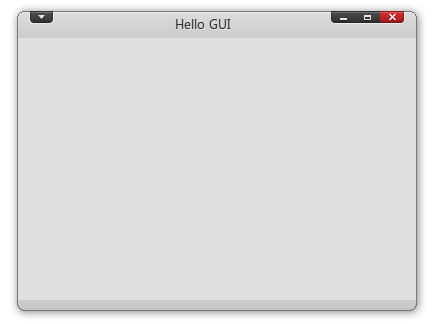
\includegraphics[width=0.6\textwidth]{fig01.png}
%% \end{figure}
% TKS %%%%%%%%%%%%%%%%%%%%%%%%%%%%%%%%%%%%%%%%%%%%%%
\begin{frame}
\centering
{\Huge \textcolor{blue}{THE END}} \\
\vspace{5mm}
{\Large wxd2870@163.com} \\
\end{frame}
%%%%%%%%%%%%%%%%%%%%%%%%%%%%%%%%%%%%%%%%%%%%%%%%%%
\end{document}
